\documentclass[a4paper]{book}
\usepackage{graphicx}
\title{Fundamentals of Financial Forecasting}
\begin{document}
\chapter{Introduction}
A typical goal in the financial arena is to attempt to predict the future based upon knowledge of the past, in order to make profitable trades.
In this document, we shall look primarily at the analysis of financial timeseries data, in particular the prices of stocks.
For illustrative purposes, most of our examples will be drawn from the analysis of the price history of just a few stocks, as shown
in Figure~\ref{fig:stock-prices}. Of course, in practice one must collect and analyse a large amount of data for a wide variety of stocks, 
in order to obtain more general and robust predictive models.

\chapter{Basic Time-Series Modelling}

\section{Predictive Models}
Consider the stock prices shown in Figure~\ref{fig:stock-prices},
which vary daily over a period of time.
Each sequence of prices for a given stock forms a time-series.
Here let $V(t)$ be the price of a given stock at time $t$. In general,
$V(t)$ represents the time-varying value of any asset. We
consider only the gross, not net, asset value, and hence may assume that $V(t)\ge 0$.
\begin{figure}[hbt]
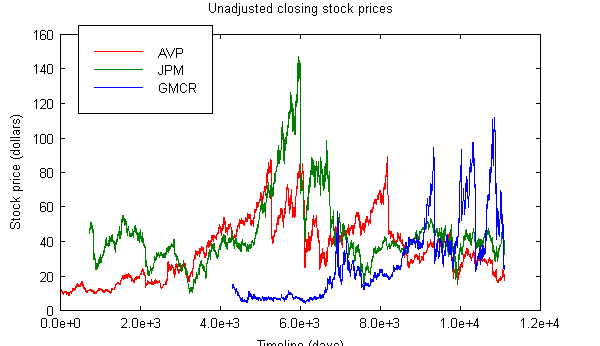
\includegraphics[scale=0.8]{figures/stock-prices-close.png}
\caption{Example data showing the unadjusted closing prices of three different
types of stock.}
\label{fig:stock-prices}
\end{figure}

Now, the purpose of a predictive model is to attempt to predict
a future value $V(t+T)$ of an asset
from knowledge of the current asset value
$V(t)$. Thus, one might begin with a Taylor series expansion
of $V(t)$, to obtain
\begin{eqnarray}
%\hspace*{-5mm}
V(t+T) & = & V(t)+V'(t)T
+V''(t)\frac{^T2}{2}
+V'''(t)\frac{T^3}{3!}
+\cdots\,,
\label{eq:Taylor-V}
\end{eqnarray}
where $V'(t)$ is the derivative of $V(t)$, etc.
The simplest such model makes use of the Mean Value Theorem
(see Appendix~\ref{sec:mean-value-theorem}) to obtain
the additive model
\begin{eqnarray}
V(t+T) & = & V(t)+V'(\xi)T
\hspace*{5mm}\mbox{for some}\,\, \xi\in[t,t+T]\,.
\label{eq:simple-additive}
\end{eqnarray}
Now, suppose for the purpose of illustration that
we buy an asset at time $t$ for amount $V(t)$ and then sell it at a later
time $t+T$ for value $V(t+T)$. Then the difference in asset values is the
{\em profit}, or {\em return}, on our investment, namely
\begin{eqnarray}
  P(t,t+T) & = & V(t+T)-V(t)~=~V'(\xi)T\,,
\end{eqnarray}
as shown in Figure~\ref{fig:avp-price-diff}.
\begin{figure}[hbt]
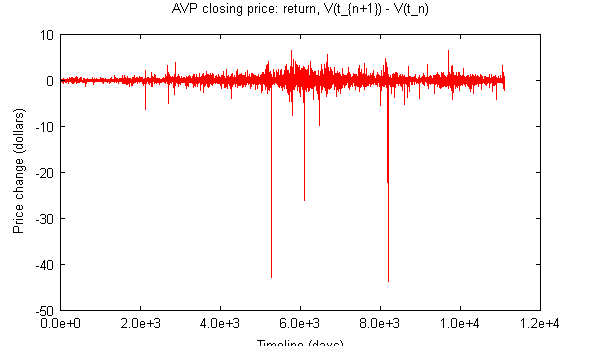
\includegraphics[scale=0.8]{figures/avp-price-close-diff.png}
\caption{Example time-series of the daily return in closing price
of AVP stock.}
\label{fig:avp-price-diff}
\end{figure}

We observe that the return has the same currency units as
the asset value. As an alternative, we might instead 
consider the profit per unit of investment, which is
a dimensionless measure 
known as the {\em relative return}, given by
\begin{eqnarray}
  Q(t,t+T) & = & \frac{P(t,t+T)}{V(t)}~=~\frac{V'(\xi)T}{V(t)}\,.
\end{eqnarray}
An example of the relative return 
is shown in Figure~\ref{fig:avp-price-simple}.
\begin{figure}[hbt]
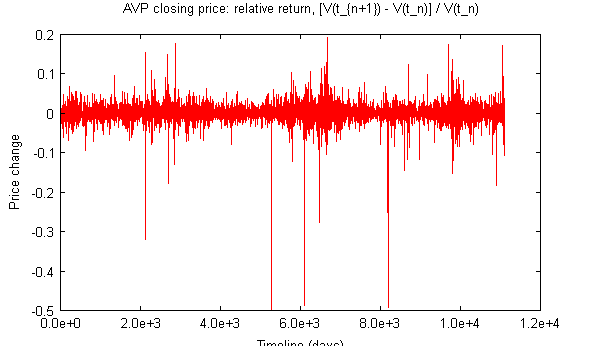
\includegraphics[scale=0.8]{figures/avp-price-close-simple.png}
\caption{Example time-series of the daily relative return of
the closing price of AVP stock.}
\label{fig:avp-price-simple}
\end{figure}

Of more use, however, is the {\em rate of return}, which is
the relative return on the investment per unit time, given by
\begin{eqnarray}
  R(t,t+T) & = & \frac{Q(t,t+T)}{T}~=~\frac{V'(\xi)}{V(t)}\,,
\end{eqnarray}
as show in Figure~\ref{fig:avp-price-log}.
Now, in the limit as $T\rightarrow 0$, observe that $\xi\rightarrow t$, and
hence the rate of return reduces to
\begin{eqnarray}
  r(t) & = & \lim_{T\rightarrow 0}R(t,t+T) ~=~\frac{V'(t)}{V(t)}\,,
\label{eq:inst-rate-return}
\end{eqnarray}
which is known as the {\em instantaneous rate of return}.
\begin{figure}[hbt]
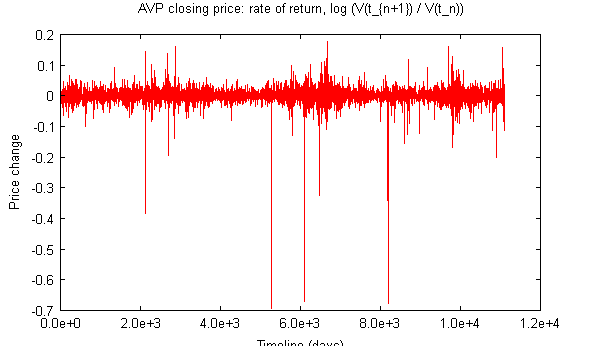
\includegraphics[scale=0.8]{figures/avp-price-close-log.png}
\caption{Example time-series of the daily rate of return of
the closing price of AVP stock.}
\label{fig:avp-price-log}
\end{figure}

In order to relate $r(t)$ back to the predictive model of $V(t+T)$,
first note that although $V(t)\in[0,\infty]$ has a restricted range,
$\ln V(t)\in(-\infty,\infty)$ has an unrestricted range, which is
a very useful property in modelling terms.
Thus, following along the lines of equation~(\ref{eq:Taylor-V}),
we turn to a Taylor series expansion
of $\ln V(t)$ to obtain
\begin{eqnarray}
%\hspace*{-6mm}
\ln V(t+T) & = & \ln V(t)+\frac{V'(t)}{V(t)}T
+\left[\frac{V''(t)}{V(t)}
-\frac{V'(t)^2}{V(t)^2}\right]
\frac{T^2}{2}
+\cdots\,.
\label{eq:Taylor-log-V}
\end{eqnarray}
This in turn (again via the Mean Value Theorem)
reduces to the log-additive model
\begin{eqnarray}
\ln V(t+T) & = & \ln V(t)+T\frac{V'(\xi)}{V(\xi)}
\hspace*{5mm}\mbox{for some}\,\, \xi\in[t,t+T]\,.
\end{eqnarray}
Hence, from equation~(\ref{eq:inst-rate-return}), we see that
\begin{eqnarray}
\ln V(t+T)~=~\ln V(t)+T\;r(\xi) & \Leftrightarrow &
V(t+T) ~=~V(t) \;e^{T\;r(\xi)}\,.
\label{eq:rate-model}
\end{eqnarray}
As a consequence, $r(t)$ is also known as the
{\em logarithmic rate of return}, and has
the unrestricted range $r(t)\in(-\infty,\infty)$. In addition,
we note that
\begin{eqnarray}
\lim_{N\rightarrow\infty}\left(1+\frac{r(t)}{N}\right)^{N} & = &
e^{r(t)}\,,
\end{eqnarray}
and so $r(t)$ is also called the
{\em continuously compounded rate of return}.

\section{Stochastic Models}

Consider the rate of return model developed in the previous
section, given by equation~(\ref{eq:rate-model}).
We note that the logarithmic return over the interval $[t,t+T]$
is given by $T\;r(\xi)$ for some $\xi\in[t,t+T]$.
Since the value of $\xi$ is unknown, we can treat it as a random variable,
and by extension $r(\xi)$ is also random.
Now, the model was derived using the Mean Value Theorem
(see Appendix~\ref{sec:mean-value-theorem}), which states
that $r(\xi)$ is the mean value of $r(t)$ over the interval $[t,t+T]$.
Hence, we make this dependence upon the time interval explicit
by rewriting equation~(\ref{eq:rate-model}) as
\begin{eqnarray}
\ln V(t+T) & = & \ln V(t)+T\;\bar{R}(t,t+T)\,.
\label{eq:mean-rate-model}
\end{eqnarray}
Finally, since $\bar{R}(t,t+T)$ is now considered to be
a random variable, it remains to decide how to model
its stochastic distribution.

In order to do this, first reconsider
the stock prices shown in Figure~\ref{fig:stock-prices}.
Although the value $V(t)$ of an asset is assumed to vary continuously with time $t$, the example stock prices were in
fact sampled at the close of each day of trading.
Thus, the length of time $T$ between samples,
sometimes known as a {\em bar}, is here equal to 1 day.
We therefore suppose for convenience that $\bar{R}(t,t+1)$
is distributed according to some distribution $D$ with mean
$\mu$ and variance $\sigma^2$, viz
\begin{eqnarray}
  \bar{R}(t,t+1) & \sim & D(\mu,\sigma)\,,
\end{eqnarray}
such that
\begin{eqnarray}
  \mbox{E}[\bar{R}(t,t+1)]~=~\mu, && 
\mbox{Var}[\bar{R}(t,t+1)]~=~\sigma^2\,.
\end{eqnarray}
Next, observe that the general interval $[t,t+T]$ can be partitioned into
two sub-intervals, e.g.
\begin{eqnarray}
[t,t+T] & = & \left[t,t+\frac{T}{2}\right]\bigcup 
\left[t+\frac{T}{2},t+T\right]\,.
\end{eqnarray}
Thus, from equation~(\ref{eq:mean-rate-model}), we obtain
\begin{eqnarray}
(T/2)\;\bar{R}(t,t+T/2) & = & \ln V(t+T/2) - \ln V(t)\,,\\
(T/2)\;\bar{R}(t+T/2,t+T) & = & \ln V(t+T) - \ln V(t+T/2)\,,\\
\Rightarrow T\;\bar{R}(t,t+T) & = & \ln V(t+T) - \ln V(t)
\nonumber\\
& = & \frac{T}{2}\{\bar{R}(t,t+T/2)+\bar{R}(t+T/2,t+T)\}
\,.
\end{eqnarray}
We now suppose that $\bar{R}(t,t+T/2)$ and $\bar{R}(t+T/2,t+T)$
are independent variables. We furthermore invoke a presumption

Thus, rather than knowing $V(t)$ for all $t$, we only know
a finite set of values $V(t_i)$ at fixed times $t_i=t_0+i\delta t$,
for $i=0,1,\ldots,n$. 
The problem then becomes one of predicting, for example, $V(t_n)$
based on knowledge of the history $V(t_i)$ for $i=0,1,\ldots,n-1$.

In our example, 

******
Suppose from equation~(\ref{eq:rate-model}) we set $t=t_{n-1}$
and $T=\delta t$. Then we obtain a predictive model of $V(t_n)$
given $V(t_{n-1})$ via
\begin{eqnarray}
\ln V(t_n) & = & \ln V(t_{n-1})+\delta t\;r(\xi_{n})\,,
\end{eqnarray}
where $\xi_n\in[t_{n-1},t_{n}]$ is unknown.
Now, recursing backward one step, we then obtain the expansion
\begin{eqnarray}
\ln V(t_n) & = & [\ln V(t_{n-2})+\delta t\;r(\xi_{n-1})]
+\delta t\;r(\xi_{n})\,.
\end{eqnarray}
Thus, after repeated recursion, we end with the expansion
\begin{eqnarray}
\ln V(t_n) & = & \ln V(t_{0})+\delta t\;[
\;r(\xi_{1})+r(\xi_{2})+\cdots+r(\xi_{n})]\,.
\label{eq:rate-micro}
\end{eqnarray}
Alternatively, we could start again with
equation~(\ref{eq:rate-model}) and set $t=t_{0}$
and $T=n\delta t$, thereby obtaining
\begin{eqnarray}
\ln V(t_n) & = & \ln V(t_{0})+n\delta t\;
r(\xi_{n}^{*})\,,
\label{eq:rate-macro}
\end{eqnarray}
where $\xi_{n}^{*}\in[t_0,t_n]$.
Thus, by equating models~(\ref{eq:rate-micro}) and
(\ref{eq:rate-macro}), we obtain the relation
\begin{eqnarray}
r(\xi_{n}^{*}) & = & 
\frac{r(\xi_{1})+r(\xi_{2})+\cdots+r(\xi_{n})}{n}\,.
\end{eqnarray}

***blah***
\begin{eqnarray}
r(\xi_i) & \sim & D(\mu,\sigma)\,,
\end{eqnarray}
where
\begin{eqnarray}
\mu~=~E[r(\xi_i)] &,&  \sigma^2~=~Var[r(\xi_is)]\,.
\end{eqnarray}

%%%%%%%%%%%%%%%%%%%%%%%%%%%%%

\chapter{Appendix}
\section{Mean Value Theorem}
\label{sec:mean-value-theorem}
The Mean Value Theorem states that the average value of a function
$f(x)$ over the interval $x\in[a,b]$ is given by $f(\xi)$ at some
point $\xi\in[a,b]$.
Mathematically, if $f(x)$ is an integrable function
then the theorem implies that
\begin{eqnarray*}
f(\xi)~=~\frac{1}{b-a}\int_{a}^{b}f(x)\;dx
& \Leftrightarrow &
\int_{a}^{b}f(x)\;dx~=~(b-a)f(\xi)\,.
\end{eqnarray*}
Graphically, the latter relation implies that
the area under the curve over an interval
is equal to a rectangular area on the same interval,
where the height of the rectangle is just the mean value $f(\xi)$.
Alternatively, since $f(x)$ is integrable, consider its indefinite
integral
\begin{eqnarray*}
\int f(x)\;dx & = & F(x)+c\,,
\end{eqnarray*}
where $c$ is an arbitrary constant.
Then the theorem states that
\begin{eqnarray*}
F(b)-F(a) & = & (b-a)\;F'(\xi)\,,
\end{eqnarray*}
where $F'(x)=f(x)$.

%%%%%%%%%%%%%%%%%%%%%%%%%%%%%

\end{document}
